\section{Approximation of Z-rotation Using Clifford+T}

\subsection{Overview of the Algorithm}

Building on the exact synthesis algorithm of Kliuchnikov et al. \cite{exact-clifford+t}, Ross and Selinger \cite{ross} proposed an efficient algorithm to use Clifford + $T$ gates to approximate single qubit $Z$-rotation in the following form 

$$
	R_z(\theta) = \begin{pmatrix}
		e^{-i\theta/2} & 0 \\
		0 & e^{i\theta/2} \\
	\end{pmatrix}.
$$

They showed that for all $\epsilon$, there exists a Clifford + $T$ circuit $U$ in the form of 
\begin{equation}\label{ross-form}
U = \begin{pmatrix}
	a & -b^\dagger \\ 
	b & a^\dagger
\end{pmatrix}
\end{equation}
such that $\|R_z (\theta) - U \| < \epsilon$.
By the results of Kliuchnikov et al., $a \in \Z[\sq, i]$. 
The insight of Ross and Selinger is that to find such $a, b \in \mathbb{C}$ (or show no such exists) with $\lde(a) = n$ is equivalent to solving the solving the following two problems:
\begin{enumerate}
	\item To find a possible value for $a$ is equivalent to enumerate a certain finite set in $\mathbb{R}^2$
	\item To find the corresponding $b$ is equivalent to solve a the Diophantine equation in $aa^\dagger + bb^\dagger = 1$.
\end{enumerate}
Both the enumeration of and solving the Diophantine equation takes polynomial time in $n$.
The algorithm starts with $n = 0$ and keep increasing $n$ until it finds a solution.
By an number-theoretical argument, they shows that the expected time this algorithm terminates is polynomial in $\log(1/\epsilon)$, and the resulting circuit has $T$-count at most $3 \log_2(1/\epsilon) + O(\log(\log(1/\epsilon)))$.

The detailed steps are shown in the following section.

\subsection{Details of the Algorithm}

\subsubsection{Two-dimensional Grid Enumeration}

Let us first consider the field $\Z[\omega]$, where $\omega = e^{\pi i/4}$.
We have the following equality
\begin{align*}
	\omega^4 &= -1 \\ 
	\omega^5 &= -\omega = \omega^{3 \dagger} \\
	\omega^6 &= -\omega^2 = \omega^{2 \dagger} \\ 
	\omega^7 &= -\omega^3 = \omega^{\dagger} \\
\end{align*}
There fore $\Z[\omega]$ is the free $\Z$-module generated by $1, \omega, \omega^2, \omega^3$.
Write $u \in \Z[\omega]$ as $u = a \omega^3 + b \omega^2 + c \omega + d$ for some $a, b, c, d \in \Z$.
Use the fact that $\omega = \frac{1}{\sqrt{2}} (1 + i)$, we have
\begin{align*}
	u &= (d + \frac{c-a}{2} \sqrt{2}) +  i (b + \frac{c+a}{2} \sqrt{2}) \\
\end{align*}
Since $c-a$ and $c+a$ have the same parity (they must both be even or both be odd), it follows that 
$$
u = \alpha + \beta \omega
$$
where $\alpha \in \Z[\sqrt{2}, i]$ and $\beta = 0, 1$.
This is summarised in the following lemma. 
\begin{lemma}\label{z-omega-form}
	Every element in $\Z[\omega]$ can be written as $\alpha$ or $\alpha + \omega$, where $\alpha \in \Z[\sqrt{2}, i]$.
\end{lemma}

Write $u \in \Z[\omega]$ as $u = a + \sqrt{2} b$, where $a, b \in \Z[i]$.
We define $u^{\bullet} = a - \sqrt{2}b$. That is, $(-)^{\bullet}$ is the unique ring automorphism of $\Z[\omega]$ that sends $\sqrt{2}$ to $-\sqrt{2}$ and fixes $i$.

We are now ready to describe Grid, the central idea of the enumeration algorithm.

\begin{definition}[Grid]
	Let $B$ be a subset of $\mathbb{C}$. The \emph{grid} of $B$ is the set of all $u \in \Z[\omega]$ such that $u^{\bullet} \in B$.
\end{definition}

Since there is a canonical isomorphism between $\mathbb{C}$ and $\mathbb{R}^2$ by identifying $x + iy$ with $(x, y)$, we can also regard the grid of $B$ as a subset of $\mathbb{R}^2$.
By adopting the convention in \cite{ross}, when describing two-dimensional grid problem, we will not distinguish between $\mathbb{C}$ and $\mathbb{R}^2$ and write $A, B$ as subsets of $\mathbb{R}^2$.

Using lemma \ref{z-omega-form}, we have the following innocuous looking lemma

\begin{lemma}[Discrete Grid]\label{discrete-grid}
	Let $U = \{(a + \sqrt{2} b, c + \sqrt{2} d)\}$ be subset of $\Z[\omega]$ where $a, b$ have the same sign, while $c, d$ have the same sign.
	Then $U$ is a discrete subset of $\mathbb{R}^2$, that is, for every bounded subset $A \subset \mathbb{R}^2$, the set $ U \cap A$ is finite.
\end{lemma}

\begin{proof}
	Using lemma \ref{z-omega-form}, any element in $\Z[\omega]$ can be written as $\alpha$ or $\alpha + \omega$, where $\alpha \in \Z[\sqrt{2} ,i]$.

	Let us first consider the case when $u = \alpha \in U$. 
	It can be written as $u = (a + b \sqrt{2}, c + d \sqrt{2})$ (where we use the canonical isomorphism to denote $\mathcal{C}$ as an element in $\mathbb{R}^2$).
	Since $u$ is in a bounded region, we may assume $|a + b\sqrt{2} | < \beta$ for some $\beta > 0$. Since $a$ and $b$, it is evident that there are only finitely many choices for $a$ and $b$.
	The same argument applies to $c$ and $d$. 

	The other case is exactly the same
\end{proof}

\begin{definition}[Two-dimensional Grid Problem]
	Let $A, B$ be subsets of $\mathbb{C}$.
	The two-dimensional grid problem for $A$ and $B$ is to find all $u \in \Z[\omega]$ such that $u \in A$ and $u^{\bullet} \in B$.
\end{definition}


An immediate observation is the following lemma. 

\begin{lemma}\label{grid-solution}
	If $B$ is a bounded convex and closed subset of $\mathbb{R}^2$ with non-empty interior and $A$ some bounded subset.
	There there exists only finitely many $u$ such that $u \in A$ and $u^{\bullet} \in B$.
\end{lemma}

\begin{proof}
	Let us try to find all $u$ such that $u \in A$ and $u^{\bullet} \in B$.

	Write $u^{\bullet} = (a + \sqrt{2} b, c + \sqrt{2} d)$. 
	Let us consider $a + \sqrt{2}b$ first. 

	There are two cases: $a, b$ have the same sign or they have different signs. 
	$u^\bullet \subset B$ and $B$ is bounded, by lemma \ref{discrete-grid} there exists only finitely many $a + \sqrt{2} b$ such that $a, b$ have the same sign and $a + \sqrt{2}b$ is in the bounded region.
	If it is in the second case, we have $u = (a - \sqrt{2} b , c - \sqrt{2}d)$. As $a, b$ are of different signs, $a, -b$ will have the same sign. Since $u \in A$ where $A$ is bounded, apply lemma \ref{discrete-grid} again, we have only finitely many choices for $a - \sqrt{2} b$.  

	The argument the the $y$ direction is the same, which completes the proof.
\end{proof}

An demonstration of the grid problem for $u \in [-5, 5] \times [-5, 5]$ and $u^\bullet [-1, 1] \times [-1, 1]$ is presented in figure \ref{fig:Demonstration of grid problem}.

\begin{figure}[htbp]
	\centering
	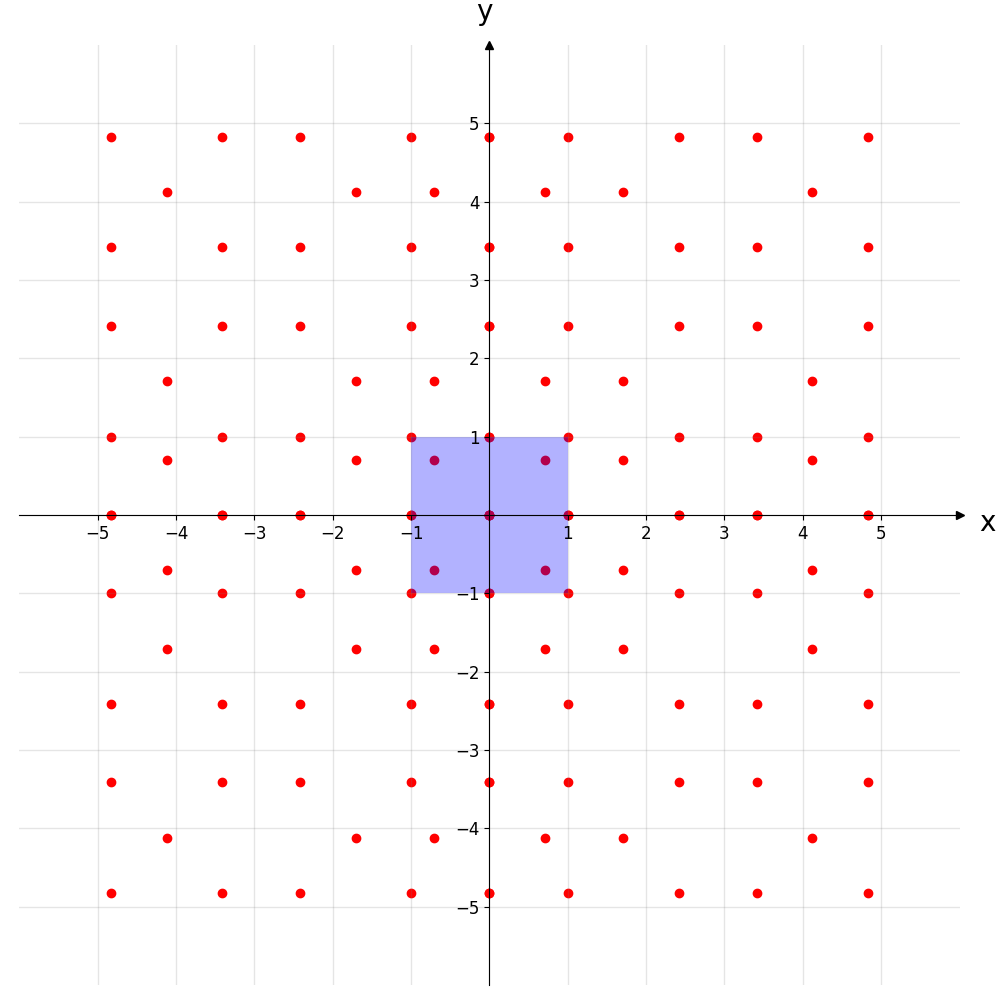
\includegraphics[width=0.6\textwidth]{./python/discrete-set.png}
	\caption{Solution to the Grid problem $u \in [-5, 5] \times [-5, 5]$ and $u^\bullet [-1, 1] \times [-1, 1]$.}
	\label{fig:Demonstration of grid problem}
\end{figure}

So for we have focused on the case when $u \in \Z[\omega]$, where the least denominator exponent of $u$ is $0$. (We used the same definition for least denominator exponent as in definition \ref{def:lde}.)
When the least denominator exponent of $u$ is some finite $n$, we can write $u = \frac{1}{\sqrt{2}^n} u'$, where $u' \in \Z[\omega]$. 
It is clear that the finiteness condition which we derived in lemma \ref{grid-solution} still holds for $u'$, so all of our arguments above can be applied to $u'$ with only minor modification.

In theorem \ref{grid-solution}, we have produced a finite set which contains all the solutions to the grid problem.
With some regularity constraints, we may assume that we can check whether a given $u$ is in the required set efficiently. \footnote{
	The details of the regularity constraints is complicated but are not too important for our discussion. Check \cite{ross} section 5.2, 5.3, 5.4 for more details.
}

This leads to central result of this section.

\begin{corollary}\label{grid-algorithm}
	For $u \in \Z[\sq, i]$ with finite least denominator exponent.
	Given a bounded convex and closed subset $B$ of $\mathbb{R}^2$ with non-empty interior and some bounded subset $A$, there is an efficient algorithm thatfinds all $u$ such that $u \in A$ and $u^{\bullet} \in B$.
\end{corollary}

From the results of \cite{exact-clifford+t}, we know that any single-qubit unitary that can be implemented by Clifford + $T$ gates must be in the form of 
\begin{equation}\label{clifford+t-form-1}
\begin{pmatrix}
	a & -b^\dagger \omega^l \\ 
	b & a^\dagger \omega^l \\
\end{pmatrix}
\end{equation}
where $a, b \in \Z[\sq, i]$, $\omega = e^{\frac{\pi}{4}}$ and $l$ is an integer. 

When approximating $R_z(\theta)$, however, we can show that $l = 0$.

\begin{lemma}
	Let $U$ be a single-qubit unitary generated by Clifford + $T$ gates. If $\|R_z{\theta} - U\| \leq |1 - e^{\frac{\pi}{8}}|$, then U must be in the form 
	\begin{equation}\label{clifford+t-form-nophase}
	\begin{pmatrix}
		a & -b^\dagger \\ 
		b & a^\dagger 
	\end{pmatrix}
	\end{equation}
	For some $a, b \in \Z[\sq, i]$.
\end{lemma}

\begin{proof}
	
\end{proof}

\subsubsection{Solving the Diophantine Equation}

